\documentclass[11pt]{article}
\usepackage[margin=1in]{geometry}
\usepackage[T1]{fontenc}
\usepackage{lmodern,amsmath,amssymb,amsthm,booktabs,graphicx,microtype}
\usepackage[hidelinks]{hyperref}
\newtheorem{proposition}{Proposition}
\newcommand{\Prob}{\mathbb P}
\newcommand{\E}{\mathbb E}
\setlength{\emergencystretch}{2em}
\title{Measured Scenario Injection for Privacy Audits:\\Search Coverage, Evidence Integrity, and Independent Confirmation}
\author{Ronald Rethabile Malamule Mahomane\\\small\texttt{ron@basisenergygroup.com}}
\date{Working manuscript, 23 October 2026}
\begin{document}
\maketitle
\begin{abstract}
A language model can propose a privacy attack scenario, but its output does not establish either that the attack works or that a release is safe. We study a constrained scenario-injection pipeline in which measured attacks supply development labels and fresh trials confirm selected findings. We compare random, domain-informed, scrambled Sobol and neural-guided search under matched evaluator budgets on 30 public Census state samples. Across 1,443,840 attack trials, Sobol search confirms 13.83 distinct high-risk scenario cells per state, compared with 10.07 for neural-guided search. The paired difference is -3.77 cells, with an exploratory state-bootstrap interval of [-4.43,-3.07]. A synthetic audit-retry experiment shows why efficient discovery and valid certification must be kept separate. We also reproduce and repair four intake or evidence-integrity defects. These experiments establish baselines and boundaries for an LLM-assisted system; no live LLM comparison is reported, and the public-file measurements do not estimate risk in an undisclosed population.
Neural search nevertheless confirms 31.57 of 32 selected configurations as high risk, compared with 22.03 for Sobol, exposing a targeting--coverage tradeoff.
\end{abstract}
\noindent\textbf{Keywords:} privacy auditing; scenario search; adaptive evaluation; evidence provenance; record linkage.

\section{Introduction}
Privacy review is a search problem as well as an inference problem. An analyst can vary release coarsening, minimum cell sizes and the adversary's auxiliary information, then learn from each observed attack. A model may help decide what to try next. A separate question is whether the evidence justifies a claim about the selected scenario or a release decision. The two questions require different evaluation criteria and access to different evidence.

Our motivating architecture uses an LLM as a constrained injector into a numerical risk model. The generator supplies a scenario description and schema-checked actions. A reviewer and a fixed evaluator determine whether it can become measured development evidence. Model predictions guide search; they are not attack counts, confidence bounds or release authority. Here ``closed'' describes this restricted data path. It does not mean an air-gapped system, fixed model weights, or a proof of privacy.

We contribute an executable, budget-matched public-file comparison; a conditional confirmation argument for adaptively selected scenarios; and regression evidence for four integrity defects in a prototype. The main empirical finding is negative: neural-guided risk targeting covers fewer confirmed high-risk cells than a space-filling baseline. The data support separating coverage from predicted severity. They do not yet support an LLM superiority claim.

\section{Related work and scope}
FunSearch couples language-model proposals with a systematic evaluator, and AlphaEvolve extends evaluator-guided search to algorithms and computational systems \cite{funsearch,alphaevolve}. This generator--evaluator pattern is therefore prior work, not our novelty claim. Curiosity-driven red teaming explicitly addresses the coverage limits of generators that find only a narrow range of successful cases \cite{curiosity}. Our evaluated target is a declared record-linkage attack on public empirical files, rather than harmful text from an LLM.

Adaptive data analysis explains why a test set cannot be treated as untouched after repeated feedback \cite{holdout}. Recent adaptive AI auditing uses e-processes to obtain anytime-valid conclusions \cite{zhou}. We use fixed-size fresh confirmation draws in the public-file experiment. Its finite-family conditional union bound is elementary; it is not a new theorem about arbitrary adaptive sampling. Formal differential privacy, unknown attacks and population identification risk are outside the claims made here.

\section{Architecture and threat model}
The intended sequence is proposal, schema validation, documented review, measured development outcomes, model fitting, selection freeze and independent confirmation. The model sees numerical features and observed counts. It does not execute proposal prose. In particular, generating an interesting description does not add an executable attack family: that requires a separately implemented evaluator.

The evaluated search strategies choose configurations from a fixed catalogue, not new attack algorithms. A proposal varies Public Use Microdata Area (PUMA) coarsening, education coarsening, minimum released cell size and auxiliary-income noise. Features include release retention, reciprocal key frequency, log file size and the declared action settings. No final confirmation outcome enters the search history.

We assume a correct evaluator and honest logging for the statistical experiment. The current local implementation does not enforce those assumptions against an operator who controls its key, file system and caller-supplied evidence. Provenance is optional; a service-issued evidence identity, durable budget reservation and external chain anchoring remain deployment requirements.

\section{Methods}
\subsection{Public empirical files and the declared attack}
We load the 29,501-row \texttt{census2000} public-use extract distributed with the Python \texttt{wooldridge} package. The source documentation attributes the extract to the US Census Bureau through Alberto Abadie \cite{wooldridge}. The experiment selects the first 30 encoded state groups containing at least 100 rows, before observing attack outcomes. This is a convenience subset of the released extract, not a national probability sample or a sample of confidential registers.

A released key uses state, PUMA, coarsened education and experience in ten-year bands. PUMA widths are $1,10,100$; education widths are $1,2,4,8$; minimum cell counts are $1,3,5,10$; and the standard deviation of the auxiliary log-income reading is $0.1,0.25,0.5,1,2$. Settings releasing fewer than 30 records are excluded. There are at most 240 settings before warm-start exclusion.

For each trial a target is sampled uniformly with replacement from the released file. An auxiliary income reading is the target's public-file log income plus fresh Gaussian noise. The attacker assigns prior weight $0.9$ to matching keys and $0.1/(n-1)$ to other records, multiplies by the Gaussian reading likelihood, and selects the maximum-weight record. We implement the calculation in log space. Success means matching the target's empirical record index. Conditional on a fixed file and scenario, fresh target and noise draws define the Bernoulli trial law. No claim about the hidden population follows from this conditional experiment.

\subsection{Search budget and coverage endpoint}
Each state block shares 16 warm-start settings measured with 64 trials each. Early stopping uses eight measured settings in the next eligible state, also with 64 trials each. These 24 settings cost 1,536 trials per block and are shared across search strategies. Every strategy then chooses 32 distinct additional settings, measured with 64 trials each, followed by 300 fresh confirmation trials for each selected setting. The overall cost is
\[
30\{24(64)+4(32)(64+300)\}=1,443,840
\]
attack trials. Model-fitting compute is not equal across strategies: the neural arm fits four models per state, whereas the other arms do not fit a model. Equal evaluator budgets do not imply equal total cost.

Random search samples without replacement. The heuristic ranks reciprocal key frequency plus $0.2/(0.1+\mathrm{sd})$. Sobol search maps a scrambled four-dimensional sequence onto the discrete action catalogue and skips duplicates. Neural search fits a two-hidden-layer ReLU model of width 16 to the counted outcomes, then acquires batches of eight by predicted risk plus 0.15 times distance to the nearest measured feature vector. The distance bonus is a fixed exploration heuristic, not a posterior uncertainty estimate. Training uses Adam and early stopping with patience 60.

The primary endpoint counts distinct scenario cells containing at least one confirmed high-risk selected configuration. A cell is the product of the three PUMA levels, education width above or below two, minimum cell count equal to one or greater, and auxiliary standard deviation above or below 0.5. There are at most 24 cells. This is a deliberately fixed coverage taxonomy; cells are not newly discovered attack families and may be correlated. The primary contrast is neural search minus Sobol search. We report descriptive paired-state bootstrap intervals from 10,000 resamples. The design was recorded before the full run but was not externally preregistered.

\subsection{Fresh confirmation after adaptive search}
Let $\mathcal D$ contain the complete development history. Conditional on $\mathcal D$, each selected configuration $i$ has a fixed attack law with risk $r_i$ and a fresh count $K_i\sim\operatorname{Binom}(300,r_i)$. We compute the one-sided Clopper--Pearson lower limit $L_i$ at level $\gamma=0.05/128$ and call the configuration high risk only when $L_i>0.2$. The 128 tests comprise 32 configurations from each of four arms within one state.

\begin{proposition}
Under the stated conditional binomial law, the probability of incorrectly confirming any configuration with $r_i\leq0.2$ is at most 0.05 within a state, even if its selection depends on the complete development history.
\end{proposition}
\begin{proof}
Conditional on $\mathcal D$, exact binomial inversion gives $\Prob(L_i>r_i\mid\mathcal D)\leq\gamma$. If $r_i\leq0.2$, then $\{L_i>0.2\}$ is contained in $\{L_i>r_i\}$. A union bound over at most 128 selected configurations gives $128\gamma=0.05$. Taking expectations over $\mathcal D$ proves the claim. Independence between different configurations is unnecessary for the union bound.
\end{proof}
The bound is per state, not simultaneously across all 30 states. This confirms excessive risk for the declared attack; it does not certify a safe release. Safety certification uses an upper bound and a different direction of inference.

\section{Results}
\subsection{Public-file discovery coverage}
\begin{table}[htbp]
\centering\small
\caption{Public-file search at the initial 600-epoch neural cap. Each arm uses 32 development queries and fresh confirmation on each of 30 state samples. Intervals are paired-state bootstrap differences from Sobol.}
\label{tab:public-search}
\begin{tabular}{lrrr}
\toprule
Search & Confirmed cells & Confirmed settings & Difference [95\% interval] \\
\midrule
Random & 13.20 & 22.50 & -0.63 [-1.23, -0.03] \\
Domain heuristic & 11.97 & 32.00 & -1.87 [-2.37, -1.33] \\
Scrambled Sobol & 13.83 & 22.03 & +0.00 [+0.00, +0.00] \\
Neural search & 10.07 & 31.57 & -3.77 [-4.43, -3.07] \\
\bottomrule
\end{tabular}
\end{table}

With the initial 600-epoch cap, Sobol search confirms 13.83 cells per state; random search 13.20; the informed heuristic 11.97; and neural search 10.07. The neural-minus-Sobol difference is -3.77 cells (paired-state interval -4.43 to -3.07). These bootstrap intervals describe variation among the selected public-file states and are not a design-based estimate for all states or institutions. Four of the 120 neural fits reach the best-epoch cap, so a larger-cap sensitivity run is reported separately rather than called convergence.

At a 2,000-epoch cap the neural mean remains 10.07 cells and the difference from Sobol is -3.77 [-4.40, -3.07]. There are 0 best-epoch cap hits, but the maximum best epoch is 1999; absence of a best-epoch cap hit is not proof of convergence. This sensitivity run reuses the same state files, warm starts, stopping evidence and non-neural draws; it is not independent replication.

The complementary endpoint shows the targeting--coverage tradeoff: neural search confirms 31.57 of its 32 selected settings as high risk on average, compared with 22.03 for Sobol. The simple informed heuristic confirms all 32 on average. These are descriptive secondary results, and confirmation of many related configurations does not establish discovery of many attack families. The informed heuristic is therefore a necessary control for any future claim that neural targeting adds value.
\begin{figure}[htbp]
\centering
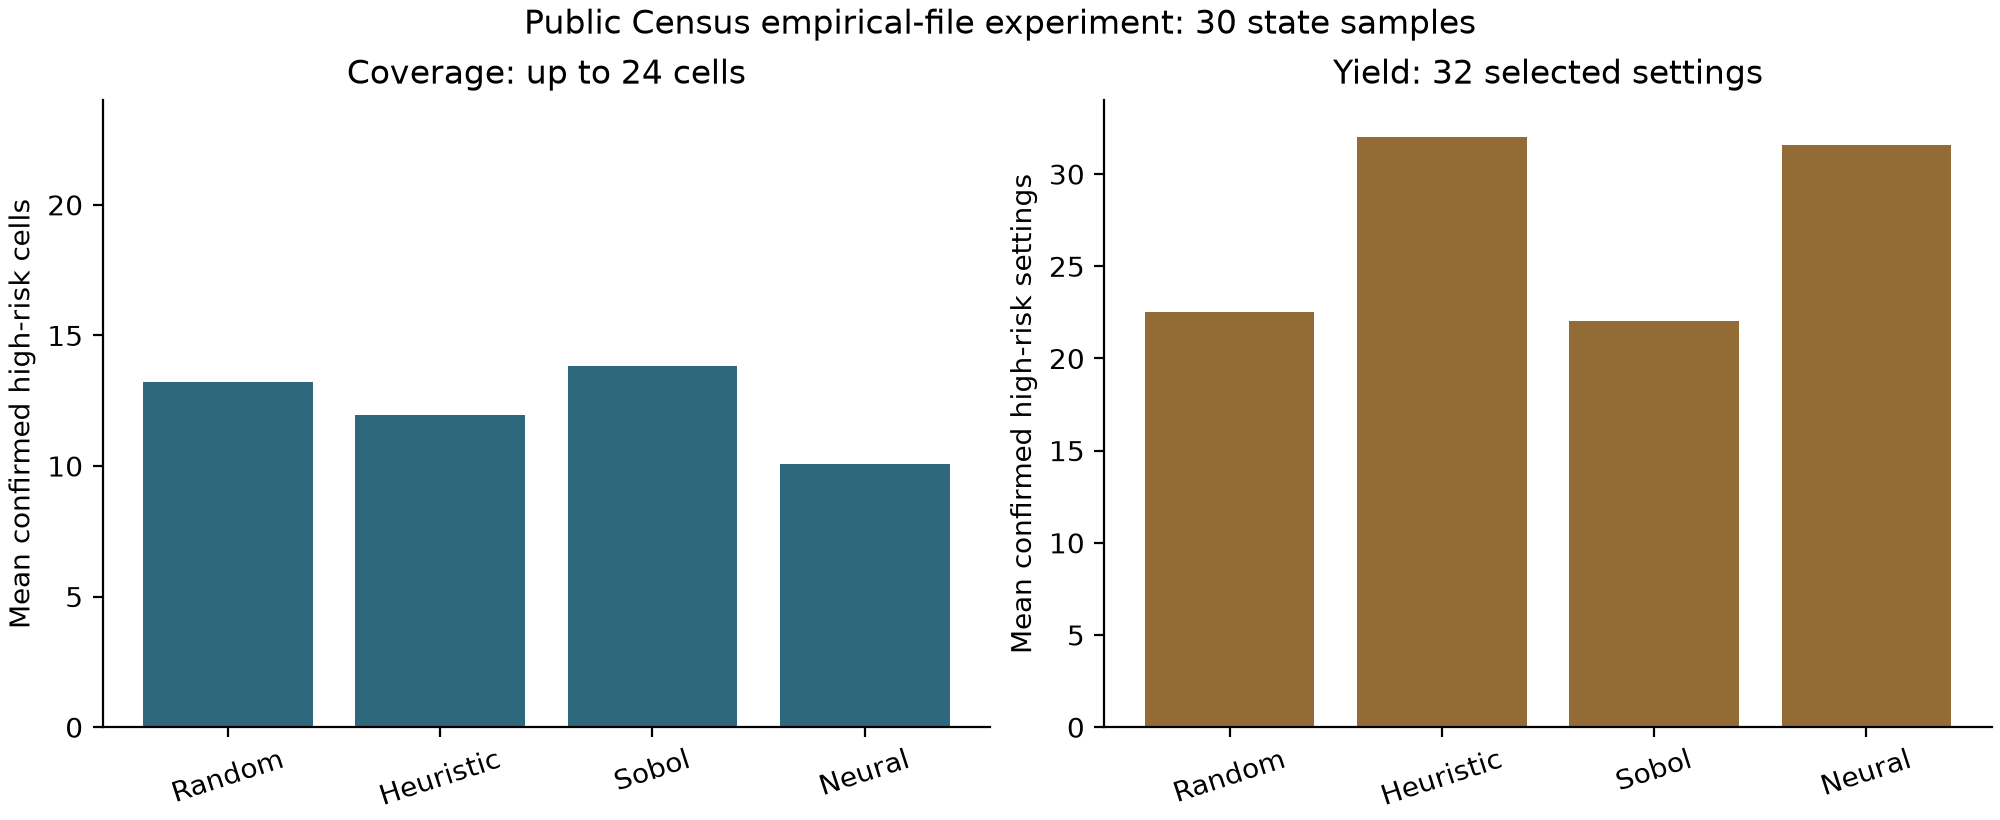
\includegraphics[width=\linewidth]{generated/public_search.png}
\caption{Matched-budget public-file scenario search. Left: mean confirmed high-risk cells. Right: mean confirmed high-risk selected settings. Table~\ref{tab:public-search} reports differences from Sobol and paired-state intervals. Targeting yield and cell coverage give different rankings. The LLM arm has not been run.}
\end{figure}

\subsection{Predictive pilots and audit retries}
Two earlier synthetic pilots provide context rather than independent confirmation of the public-file result. A probability-law experiment used ten seeds and 120 model fits; a synthetic nearest-record experiment used five seeds, 1,382,000 executed linkage trials and 30 fits. On the latter, random augmentation changed the deep model's shifted-test log loss by -0.0133 (95\% seed-level interval -0.0342 to 0.0075). Heuristic augmentation changed it by -0.0127 (-0.0331 to 0.0077). Neither establishes an improvement. These exploratory intervals are not multiplicity-adjusted.

A separate synthetic boundary experiment tests repeated safety certification. True risk is 0.201, tolerance 0.2, and each attempt uses 500 independent trials. Among 20,000 simulated programmes with 20 attempts each, resetting the nominal level to 0.05 gives 50.975\% false certification; preallocating a total 0.05 budget across attempts gives 3.875\%. Exact binomial intervals are [50.280\%,51.670\%] and [3.612\%,4.152\%]. The result illustrates repeated-selection error under the simulated law. It does not demonstrate that the local ledger can stop an operator from obtaining and discarding unrecorded outcomes.

\subsection{Evidence-integrity regression experiment}
Four regression probes fail against the supplied prototype: altered measured counts are accepted, altered measured features are accepted, an injected copy can match validation features after identifier changes, and file-intake metadata can bypass the response-size limit. Repairs commit the full measured row's digest to the keyed chain, check that commitment at training-artifact acceptance, conservatively reject identical injected validation vectors, and bound file input before JSON parsing. The copy rule can reject legitimate feature collisions and does not detect semantic contamination. The original validation snapshot reports 178 passing tests and 91.57\% source coverage; the new search tests and updated full-suite validation are recorded with this revision.

The updated revision passes 183 tests with 90.58\% source coverage; Ruff reports no violations. The full test log accompanies the revision. These software checks do not establish statistical sampling assumptions or authenticate an external evaluator.

\section{Interpretation and limitations}
The public-file result rejects a convenient assumption: increasing model sophistication does not necessarily improve failure coverage. A predictor can be useful for high-yield targeting while repeatedly choosing related settings. Our coverage score also favors space filling by construction, so a complete assessment must report the number and severity of confirmed candidates alongside cell coverage, and compare with diversity-aware heuristic controls. We do not infer neural inferiority for all objectives from this one endpoint.

The live LLM arm is absent. No result here measures the contribution of generated language, newly proposed attack families, model-provider differences or the cost of model calls. The study is an evaluation foundation for that claim. A future comparison must record exact prompts, provider model versions, rejection rates, retry rules and complete generation costs before reading confirmation outcomes.

The experiment uses one public extract and one attacker, with declared coarsening choices and simulated auxiliary noise. Log-income readings are modeling assumptions. Synthetic auxiliary observations on real records do not constitute measurements from an operational adversary. Source records and conditional targets are not independent institutional programmes, and the 30-state subset does not identify population confidentiality. The catalogue omits longitudinal pooling, attribute inference and unknown attacks.

The provenance implementation remains a local prototype. Full-row hashes deter substitution only when lineage and ledger use are retained. A key holder can rewrite a chain; an unauthenticated caller can relabel base evidence; and budget debits after supplied outcomes do not prevent withholding. A deployment needs an independently controlled evaluator, transactional reservations before draws, an append-only registry and external anchoring.

The coverage taxonomy measures diversity of declared configurations, not semantic diversity of attacks. Different coarsening choices can induce identical partitions in a particular empirical file, and some cells are infeasible after suppression. All methods use the same available catalogue within a state, but the score should not be interpreted as a universal measure of security coverage. The next comparison should include partition-equivalence checks and diversity-aware controls.

\section{Next experiment and conclusion}
The immediate empirical gate is a genuine LLM-versus-Sobol comparison using the same executable evaluator and budgets, followed by a diversity-aware heuristic control. The next external-validity gate is a second public dataset with an independently specified attacker. These should be locked before confirmation outcomes are inspected. We have no basis yet to claim either LLM superiority or deployment readiness.

The current result is narrower but useful: measured scenario injection can be tested reproducibly, simple search is competitive on a real public-file substrate, and evidence integrity and statistical confirmation impose constraints that prediction quality alone cannot satisfy.

\section*{Reproducibility and overlap}
Code and aggregate scenario measurements are in \url{https://github.com/Nube1/privacy-risk-thresholds}, branch \texttt{codex/llm-injector-evaluation}. The repository is currently private; public reproducibility requires making an appropriately reviewed release accessible. The source-data snapshot hash, design, state-level counts and results are recorded with the experiments. This draft extends an existing working manuscript on programme-level privacy risk and a separate journal draft on adaptive certification. Their carried-over theory and synthetic findings are not presented here as new independent results. This is an author manuscript, not a publisher-issued article.

\begin{thebibliography}{9}
\bibitem{funsearch} Romera-Paredes, B. et al. (2024). Mathematical discoveries from program search with large language models. \emph{Nature} 625, 468--475. \url{https://doi.org/10.1038/s41586-023-06924-6}.
\bibitem{alphaevolve} Novikov, A. et al. (2025). AlphaEvolve: A coding agent for scientific and algorithmic discovery. \url{https://arxiv.org/abs/2506.13131}.
\bibitem{curiosity} Hong, Z.-W. et al. (2024). Curiosity-driven Red-teaming for Large Language Models. \emph{ICLR}. \url{https://arxiv.org/abs/2402.19464}.
\bibitem{holdout} Dwork, C. et al. (2015). Generalization in Adaptive Data Analysis and Holdout Reuse. \url{https://arxiv.org/abs/1506.02629}.
\bibitem{zhou} Zhou, S., Vossler, P., Sivaraman, V., Mai, Y. and Feng, J. (2026). Adaptive auditing of AI systems with anytime-valid guarantees. Preprint. \url{https://arxiv.org/abs/2605.07002}.
\bibitem{wooldridge} Wooldridge data package. \texttt{census2000} documentation and source attribution. \url{https://cran.r-project.org/web/packages/wooldridge/wooldridge.pdf}. Python package version used: 0.5.0; source snapshot hash supplied with the experiment.
\end{thebibliography}
\end{document}
